\documentclass{article}
\usepackage[utf8]{inputenc}
\usepackage[top=1in]{geometry}
\usepackage{graphicx}
\usepackage{booktabs}
\usepackage{amsmath}
\usepackage{amsthm}
\usepackage[only]{excludeonly}
\usepackage{tikz}
\usetikzlibrary{circuits.logic.US,positioning,calc} 
% https://tex.stackexchange.com/questions/140567/drawing-karnaughs-maps-in-latex
\usepackage{tikz}
\usetikzlibrary{matrix,calc}

%isolated term
%#1 - Optional. Space between node and grouping line. Default=0
%#2 - node
%#3 - filling color
\newcommand{\implicantsol}[3][0]{
    \draw[rounded corners=3pt, fill=#3, opacity=0.3] ($(#2.north west)+(135:#1)$) rectangle ($(#2.south east)+(-45:#1)$);
    }


%internal group
%#1 - Optional. Space between node and grouping line. Default=0
%#2 - top left node
%#3 - bottom right node
%#4 - filling color
\newcommand{\implicant}[4][0]{
    \draw[rounded corners=3pt, fill=#4, opacity=0.3] ($(#2.north west)+(135:#1)$) rectangle ($(#3.south east)+(-45:#1)$);
    }

%group lateral borders
%#1 - Optional. Space between node and grouping line. Default=0
%#2 - top left node
%#3 - bottom right node
%#4 - filling color
\newcommand{\implicantcostats}[4][0]{
    \draw[rounded corners=3pt, fill=#4, opacity=0.3] ($(rf.east |- #2.north)+(90:#1)$)-| ($(#2.east)+(0:#1)$) |- ($(rf.east |- #3.south)+(-90:#1)$);
    \draw[rounded corners=3pt, fill=#4, opacity=0.3] ($(cf.west |- #2.north)+(90:#1)$) -| ($(#3.west)+(180:#1)$) |- ($(cf.west |- #3.south)+(-90:#1)$);
}

%group top-bottom borders
%#1 - Optional. Space between node and grouping line. Default=0
%#2 - top left node
%#3 - bottom right node
%#4 - filling color
\newcommand{\implicantdaltbaix}[4][0]{
    \draw[rounded corners=3pt, fill=#4, opacity=0.3] ($(cf.south -| #2.west)+(180:#1)$) |- ($(#2.south)+(-90:#1)$) -| ($(cf.south -| #3.east)+(0:#1)$);
    \draw[rounded corners=3pt, fill=#4, opacity=0.3] ($(rf.north -| #2.west)+(180:#1)$) |- ($(#3.north)+(90:#1)$) -| ($(rf.north -| #3.east)+(0:#1)$);
}

%group corners
%#1 - Optional. Space between node and grouping line. Default=0
%#2 - filling color
\newcommand{\implicantcantons}[2][0]{
    \draw[rounded corners=3pt, opacity=.3] ($(rf.east |- 0.south)+(-90:#1)$) -| ($(0.east |- cf.south)+(0:#1)$);
    \draw[rounded corners=3pt, opacity=.3] ($(rf.east |- 8.north)+(90:#1)$) -| ($(8.east |- rf.north)+(0:#1)$);
    \draw[rounded corners=3pt, opacity=.3] ($(cf.west |- 2.south)+(-90:#1)$) -| ($(2.west |- cf.south)+(180:#1)$);
    \draw[rounded corners=3pt, opacity=.3] ($(cf.west |- 10.north)+(90:#1)$) -| ($(10.west |- rf.north)+(180:#1)$);
    \fill[rounded corners=3pt, fill=#2, opacity=.3] ($(rf.east |- 0.south)+(-90:#1)$) -|  ($(0.east |- cf.south)+(0:#1)$) [sharp corners] ($(rf.east |- 0.south)+(-90:#1)$) |-  ($(0.east |- cf.south)+(0:#1)$) ;
    \fill[rounded corners=3pt, fill=#2, opacity=.3] ($(rf.east |- 8.north)+(90:#1)$) -| ($(8.east |- rf.north)+(0:#1)$) [sharp corners] ($(rf.east |- 8.north)+(90:#1)$) |- ($(8.east |- rf.north)+(0:#1)$) ;
    \fill[rounded corners=3pt, fill=#2, opacity=.3] ($(cf.west |- 2.south)+(-90:#1)$) -| ($(2.west |- cf.south)+(180:#1)$) [sharp corners]($(cf.west |- 2.south)+(-90:#1)$) |- ($(2.west |- cf.south)+(180:#1)$) ;
    \fill[rounded corners=3pt, fill=#2, opacity=.3] ($(cf.west |- 10.north)+(90:#1)$) -| ($(10.west |- rf.north)+(180:#1)$) [sharp corners] ($(cf.west |- 10.north)+(90:#1)$) |- ($(10.west |- rf.north)+(180:#1)$) ;
}

%Empty Karnaugh map 4x4
\newenvironment{Karnaugh}[2]%
{
\begin{tikzpicture}[baseline=(current bounding box.north),scale=0.8]
\draw (0,0) grid (4,4);
\draw (0,4) -- node [pos=0.7,above right,anchor=south west] {#1} node [pos=0.7,below left,anchor=north east] {#2} ++(135:1);
%
\matrix (mapa) [matrix of nodes,
        column sep={0.8cm,between origins},
        row sep={0.8cm,between origins},
        every node/.style={minimum size=0.3mm},
        anchor=2.center,
        ampersand replacement=\&] at (0.5,0.5)
{
                       \& |(c00)| 00         \& |(c01)| 01         \& |(c11)| 11         \& |(c10)| 10         \& |(cf)| \phantom{00} \\
|(r00)| 00             \& |(0)|  \phantom{0} \& |(4)|  \phantom{0} \& |(12)|  \phantom{0} \& |(8)|  \phantom{0} \&                     \\
|(r01)| 01             \& |(1)|  \phantom{0} \& |(5)|  \phantom{0} \& |(13)|  \phantom{0} \& |(9)|  \phantom{0} \&                     \\
|(r11)| 11             \& |(3)| \phantom{0} \& |(7)| \phantom{0} \& |(15)| \phantom{0} \& |(11)| \phantom{0} \&                     \\
|(r10)| 10             \& |(2)|  \phantom{0} \& |(6)|  \phantom{0} \& |(14)| \phantom{0} \& |(10)| \phantom{0} \&                     \\
|(rf) | \phantom{00}   \&                    \&                    \&                    \&                    \&                     \\
};
}%
{
\end{tikzpicture}
}

%Empty Karnaugh map 2x4
\newenvironment{Karnaughvuit}%
{
\begin{tikzpicture}[baseline=(current bounding box.north),scale=0.8]
\draw (0,0) grid (4,2);
\draw (0,2) -- node [pos=0.7,above right,anchor=south west] {AB} node [pos=0.7,below left,anchor=north east] {C} ++(135:1);
%
\matrix (mapa) [matrix of nodes,
        column sep={0.8cm,between origins},
        row sep={0.8cm,between origins},
        every node/.style={minimum size=0.3mm},
        anchor=1.center,
        ampersand replacement=\&] at (0.5,0.5)
{
                      \& |(c00)| 00         \& |(c01)| 01         \& |(c11)| 11         \& |(c10)| 10         \& |(cf)| \phantom{00} \\
|(r00)| 0             \& |(0)|  \phantom{0} \& |(2)|  \phantom{0} \& |(6)|  \phantom{0} \& |(4)|  \phantom{0} \&                     \\
|(r01)| 1             \& |(1)|  \phantom{0} \& |(3)|  \phantom{0} \& |(7)|  \phantom{0} \& |(5)|  \phantom{0} \&                     \\
|(rf) | \phantom{00}  \&                    \&                    \&                    \&                    \&                     \\
};
}%
{
\end{tikzpicture}
}

%Empty Karnaugh map 2x2
\newenvironment{Karnaughquatre}%
{
\begin{tikzpicture}[baseline=(current bounding box.north),scale=0.8]
\draw (0,0) grid (2,2);
\draw (0,2) -- node [pos=0.7,above right,anchor=south west] {A} node [pos=0.7,below left,anchor=north east] {B} ++(135:1);
%
\matrix (mapa) [matrix of nodes,
        column sep={0.8cm,between origins},
        row sep={0.8cm,between origins},
        every node/.style={minimum size=0.3mm},
        anchor=1.center,
        ampersand replacement=\&] at (0.5,0.5)
{
          \& |(c00)| 0          \& |(c01)| 1  \\
|(r00)| 0 \& |(0)|  \phantom{0} \& |(2)|  \phantom{0} \\
|(r01)| 1 \& |(1)|  \phantom{0} \& |(3)|  \phantom{0} \\
};
}%
{
\end{tikzpicture}
}

%Defines 8 or 16 values (0,1,X)
\newcommand{\contingut}[1]{%
\foreach \x [count=\xi from 0]  in {#1}
     \path (\xi) node {\x};
}

%Places 1 in listed positions
\newcommand{\minterms}[1]{%
    \foreach \x in {#1}
        \path (\x) node {1};
}

%Places 0 in listed positions
\newcommand{\maxterms}[1]{%
    \foreach \x in {#1}
        \path (\x) node {0};
}

%Places X in listed positions
\newcommand{\indeterminats}[1]{%
    \foreach \x in {#1}
        \path (\x) node {X};
}

% Places m_{x} in listed positions
\newcommand{\phminterms}[1]{%
  \foreach \x in {#1}
  \path (\x) node {$m_{\x}$};
}

% Places m_{16+x} in listed positions
\newcommand{\phmintermssixt}[1]{%
  \foreach [evaluate={\y=int(16+\x)}] \x in {#1}
  \path (\x) node {$m_{\y}$};
}

% Calligraphic fonts
\newcommand{\calA}{{\cal A}}
\newcommand{\calB}{{\cal B}}
\newcommand{\calC}{{\cal C}}
\newcommand{\calD}{{\cal D}}
\newcommand{\calE}{{\cal E}}
\newcommand{\calF}{{\cal F}}
\newcommand{\calG}{{\cal G}}
\newcommand{\calH}{{\cal H}}
\newcommand{\calI}{{\cal I}}
\newcommand{\calJ}{{\cal J}}
\newcommand{\calK}{{\cal K}}
\newcommand{\calL}{{\cal L}}
\newcommand{\calM}{{\cal M}}
\newcommand{\calN}{{\cal N}}
\newcommand{\calO}{{\cal O}}
\newcommand{\calP}{{\cal P}}
\newcommand{\calQ}{{\cal Q}}
\newcommand{\calR}{{\cal R}}
\newcommand{\calS}{{\cal S}}
\newcommand{\calT}{{\cal T}}
\newcommand{\calU}{{\cal U}}
\newcommand{\calV}{{\cal V}}
\newcommand{\calW}{{\cal W}}
\newcommand{\calX}{{\cal X}}
\newcommand{\calY}{{\cal Y}}
\newcommand{\calZ}{{\cal Z}}

% Sets:
\newcommand{\setA}{\textsf{A}}
\newcommand{\setB}{\textsf{B}}
\newcommand{\setC}{\textsf{C}}
\newcommand{\setD}{\textsf{D}}
\newcommand{\setE}{\textsf{E}}
\newcommand{\setF}{\textsf{F}}
\newcommand{\setG}{\textsf{G}}
\newcommand{\setH}{\textsf{H}}
\newcommand{\setI}{\textsf{I}}
\newcommand{\setJ}{\textsf{J}}
\newcommand{\setK}{\textsf{K}}
\newcommand{\setL}{\textsf{L}}
\newcommand{\setM}{\textsf{M}}
\newcommand{\setN}{\textsf{N}}
\newcommand{\setO}{\textsf{O}}
\newcommand{\setP}{\textsf{P}}
\newcommand{\setQ}{\textsf{Q}}
\newcommand{\setR}{\textsf{R}}
\newcommand{\setS}{\textsf{S}}
\newcommand{\setT}{\textsf{T}}
\newcommand{\setU}{\textsf{U}}
\newcommand{\setV}{\textsf{V}}
\newcommand{\setW}{\textsf{W}}
\newcommand{\setX}{\textsf{X}}
\newcommand{\setY}{\textsf{Y}}
\newcommand{\setZ}{\textsf{Z}}

% Vectors
\newcommand{\bfa}{\mathbf{a}}
\newcommand{\bfb}{\mathbf{b}}
\newcommand{\bfc}{\mathbf{c}}
\newcommand{\bfd}{\mathbf{d}}
\newcommand{\bfe}{\mathbf{e}}
\newcommand{\bff}{\mathbf{f}}
\newcommand{\bfg}{\mathbf{g}}
\newcommand{\bfh}{\mathbf{h}}
\newcommand{\bfi}{\mathbf{i}}
\newcommand{\bfj}{\mathbf{j}}
\newcommand{\bfk}{\mathbf{k}}
\newcommand{\bfl}{\mathbf{l}}
\newcommand{\bfm}{\mathbf{m}}
\newcommand{\bfn}{\mathbf{n}}
\newcommand{\bfo}{\mathbf{o}}
\newcommand{\bfp}{\mathbf{p}}
\newcommand{\bfq}{\mathbf{q}}
\newcommand{\bfr}{\mathbf{r}}
\newcommand{\bfs}{\mathbf{s}}
\newcommand{\bft}{\mathbf{t}}
\newcommand{\bfu}{\mathbf{u}}
\newcommand{\bfv}{\mathbf{v}}
\newcommand{\bfw}{\mathbf{w}}
\newcommand{\bfx}{\mathbf{x}}
\newcommand{\bfy}{\mathbf{y}}
\newcommand{\bfz}{\mathbf{z}}


\newcommand{\bfalpha}{\boldsymbol{\alpha}}
\newcommand{\bfbeta}{\boldsymbol{\beta}}
\newcommand{\bfgamma}{\boldsymbol{\gamma}}
\newcommand{\bfdelta}{\boldsymbol{\delta}}
\newcommand{\bfepsilon}{\boldsymbol{\epsilon}}
\newcommand{\bfzeta}{\boldsymbol{\zeta}}
\newcommand{\bfeta}{\boldsymbol{\eta}}
\newcommand{\bftheta}{\boldsymbol{\theta}}
\newcommand{\bfiota}{\boldsymbol{\iota}}
\newcommand{\bfkappa}{\boldsymbol{\kappa}}
\newcommand{\bflambda}{\boldsymbol{\lambda}}
\newcommand{\bfmu}{\boldsymbol{\mu}}
\newcommand{\bfnu}{\boldsymbol{\nu}}
\newcommand{\bfomicron}{\boldsymbol{\omicron}}
\newcommand{\bfpi}{\boldsymbol{\pi}}
\newcommand{\bfrho}{\boldsymbol{\rho}}
\newcommand{\bfsigma}{\boldsymbol{\sigma}}
\newcommand{\bftau}{\boldsymbol{\tau}}
\newcommand{\bfupsilon}{\boldsymbol{\upsilon}}
\newcommand{\bfphi}{\boldsymbol{\phi}}
\newcommand{\bfchi}{\boldsymbol{\chi}}
\newcommand{\bfpsi}{\boldsymbol{\psi}}
\newcommand{\bfomega}{\boldsymbol{\omega}}
\newcommand{\bfxi}{\boldsymbol{\xi}}
\newcommand{\bfell}{\boldsymbol{\ell}}

% Matrices
\newcommand{\bfA}{\mathbf{A}}
\newcommand{\bfB}{\mathbf{B}}
\newcommand{\bfC}{\mathbf{C}}
\newcommand{\bfD}{\mathbf{D}}
\newcommand{\bfE}{\mathbf{E}}
\newcommand{\bfF}{\mathbf{F}}
\newcommand{\bfG}{\mathbf{G}}
\newcommand{\bfH}{\mathbf{H}}
\newcommand{\bfI}{\mathbf{I}}
\newcommand{\bfJ}{\mathbf{J}}
\newcommand{\bfK}{\mathbf{K}}
\newcommand{\bfL}{\mathbf{L}}
\newcommand{\bfM}{\mathbf{M}}
\newcommand{\bfN}{\mathbf{N}}
\newcommand{\bfO}{\mathbf{O}}
\newcommand{\bfP}{\mathbf{P}}
\newcommand{\bfQ}{\mathbf{Q}}
\newcommand{\bfR}{\mathbf{R}}
\newcommand{\bfS}{\mathbf{S}}
\newcommand{\bfT}{\mathbf{T}}
\newcommand{\bfU}{\mathbf{U}}
\newcommand{\bfV}{\mathbf{V}}
\newcommand{\bfW}{\mathbf{W}}
\newcommand{\bfX}{\mathbf{X}}
\newcommand{\bfY}{\mathbf{Y}}
\newcommand{\bfZ}{\mathbf{Z}}


\newcommand{\bfGamma}{\boldsymbol{\Gamma}}
\newcommand{\bfDelta}{\boldsymbol{\Delta}}
\newcommand{\bfTheta}{\boldsymbol{\Theta}}
\newcommand{\bfLambda}{\boldsymbol{\Lambda}}
\newcommand{\bfPi}{\boldsymbol{\Pi}}
\newcommand{\bfSigma}{\boldsymbol{\Sigma}}
\newcommand{\bfUpsilon}{\boldsymbol{\Upsilon}}
\newcommand{\bfPhi}{\boldsymbol{\Phi}}
\newcommand{\bfPsi}{\boldsymbol{\Psi}}
\newcommand{\bfOmega}{\boldsymbol{\Omega}}


% Blackboard Bold:
\newcommand{\bbA}{\mathbb{A}}
\newcommand{\bbB}{\mathbb{B}}
\newcommand{\bbC}{\mathbb{C}}
\newcommand{\bbD}{\mathbb{D}}
\newcommand{\bbE}{\mathbb{E}}
\newcommand{\bbF}{\mathbb{F}}
\newcommand{\bbG}{\mathbb{G}}
\newcommand{\bbH}{\mathbb{H}}
\newcommand{\bbI}{\mathbb{I}}
\newcommand{\bbJ}{\mathbb{J}}
\newcommand{\bbK}{\mathbb{K}}
\newcommand{\bbL}{\mathbb{L}}
\newcommand{\bbM}{\mathbb{M}}
\newcommand{\bbN}{\mathbb{N}}
\newcommand{\bbO}{\mathbb{O}}
\newcommand{\bbP}{\mathbb{P}}
\newcommand{\bbQ}{\mathbb{Q}}
\newcommand{\bbR}{\mathbb{R}}
\newcommand{\bbS}{\mathbb{S}}
\newcommand{\bbT}{\mathbb{T}}
\newcommand{\bbU}{\mathbb{U}}
\newcommand{\bbV}{\mathbb{V}}
\newcommand{\bbW}{\mathbb{W}}
\newcommand{\bbX}{\mathbb{X}}
\newcommand{\bbY}{\mathbb{Y}}
\newcommand{\bbZ}{\mathbb{Z}}




\title{Combinational circuit}
\author{Vikas Dhiman for ECE275}
\newtheorem{example}{Example}
\newtheorem{prob}{Problem}
\newtheorem{remark}{Remark}

\newcommand{\bx}{\bar{x}}
\newcommand{\by}{\bar{y}}
\newcommand{\bz}{\bar{z}}
\newcommand{\bA}{\bar{A}}
\newcommand{\bB}{\bar{B}}
\newcommand{\bC}{\bar{C}}

\includeonly{0912-notes}
\begin{document}
\maketitle
\section{Learning objectives}
\begin{enumerate}
\item Representing digital circuits
\item Converting between different notations: Boolean expression, logic
  networks and switching circuits
\item Converting between different logic network specifications: truth table, minterm,
  maxterms, product of sums canonical form and sum of product canonical form.
\end{enumerate}

\newpage
\section{Basic Gates and notations summary}
\rotatebox[origin=c]{90}{
\begin{tabular}{lccp{0.2\linewidth}ccc}
  \toprule
  Name & C/Verilog & Boolean expr. & Truth Table & Switching circuit & (ANSI) symbol & Venn diagram  \\
  \midrule
  AND Gate &
  \texttt{L = x1 \& x2} &
  $L = x_1 \cdot x_2 = x_1 x_2$ &
 \mbox{\begin{tabular}{cc|c}
 \toprule
 $x_1$ & $x_2$ & $x_1 \cdot x_2$ \\
 \midrule
 0 & 0 & 0 \\
 0 & 1 & 0 \\
 1 & 0 & 0 \\
 1 & 1 & 1 \\
 \bottomrule
 \end{tabular}} &
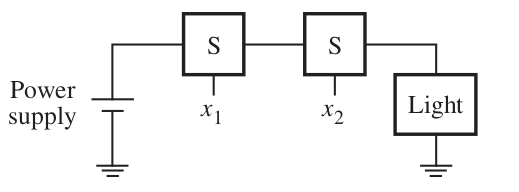
\includegraphics[width=0.2\linewidth]{AND-circuit.png} &
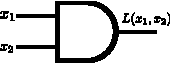
\includegraphics[width=0.2\linewidth]{AND_ANSI.pdf} &
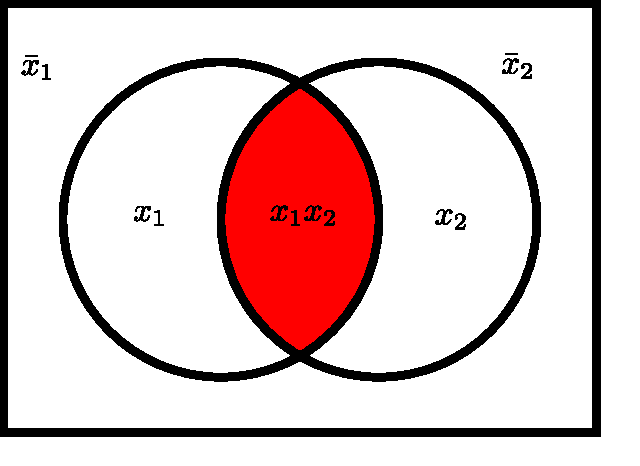
\includegraphics[width=0.2\linewidth]{AND_Venn.pdf}\\
  OR Gate &
\texttt{L = x1 | x2} &
$L = x_1 + x_2$ &
\mbox{\begin{tabular}{cc|c}
  \toprule
  $x_1$ & $x_2$ & $x_1 + x_2$ \\
  \midrule
  0 & 0 & 0 \\
  0 & 1 & 1 \\
  1 & 0 & 1 \\
  1 & 1 & 1 \\
  \bottomrule
\end{tabular}} &
\includegraphics[width=0.2\linewidth]{OR-circuit.png} &
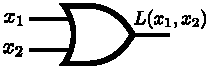
\includegraphics[width=0.2\linewidth]{OR_ANSI.pdf} & 
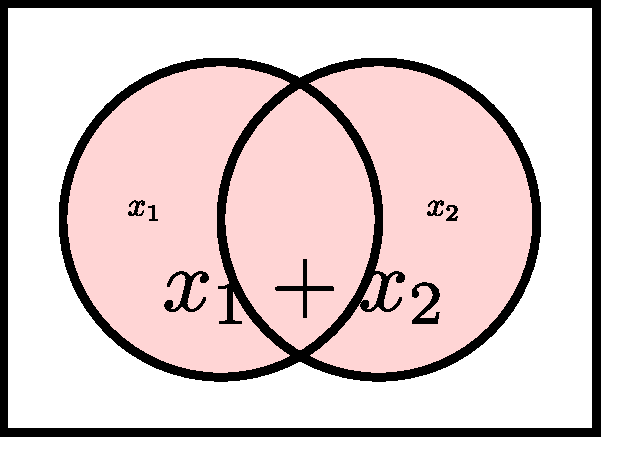
\includegraphics[width=0.2\linewidth]{OR_Venn.pdf}\\
  NOT Gate &
  \texttt{L = $\sim$ x1} &
$ L = \bar{x}_1 = x'_1$ &
\mbox{\begin{tabular}{c|c}
\toprule
$x_1$ & $\bar{x}_1$ \\
\midrule
0 & 1 \\
1 & 0 \\
\bottomrule
\end{tabular}} &
\includegraphics[width=0.2\linewidth]{NOT-circuit.png} &
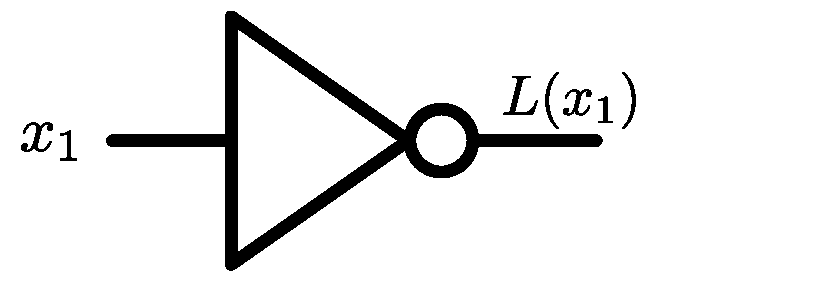
\includegraphics[width=0.2\linewidth]{NOT_ANSI.pdf} &
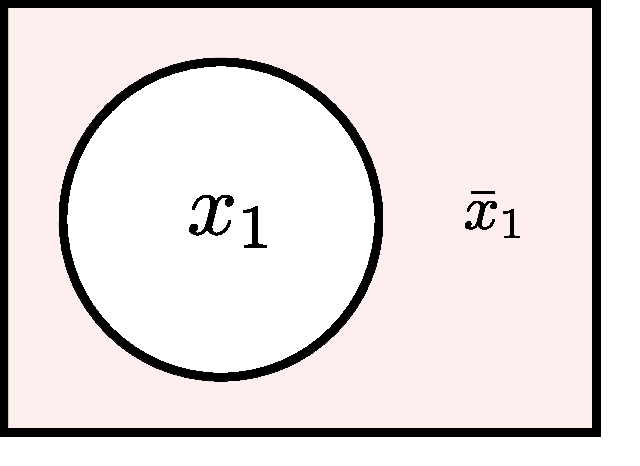
\includegraphics[width=0.2\linewidth]{NOT_Venn_x1.pdf}
\end{tabular}
}
\newpage

\section{Digital circuits or networks}

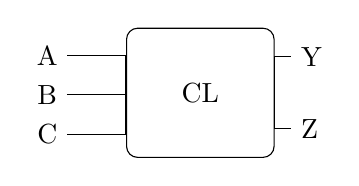
\begin{tikzpicture}[circuit logic US]
    \node (A) at (0,1) {A} ;
    \node (B) at (0,0.5) {B} ;
    \node (C) at (0,0) {C} ;
    \node [draw,rounded corners,inner sep=7mm,anchor=south west] (CL) at (1, -3mm) {CL} ; 
    \node [above right=3mm of CL.east] (Y) {Y} ;
    \node [below right=3mm of CL.east] (Z) {Z} ;

    \draw (A) -| (CL.west);
    \draw (B) -| (CL.west);
    \draw (C) -| (CL.west);
    \draw (CL.east) |- (Y);
    \draw (CL.east) |- (Z);
\end{tikzpicture}

\[
  Y = F(A, B, C) \qquad Z = G(A, B, C)
  \]

\section{Two input networks}
\begin{example}
  Convert the following (ANSI) network into a Boolean expression, a truth table
  and a Venn diagram.

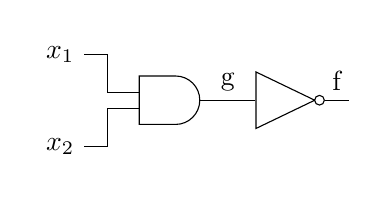
\begin{tikzpicture}[circuit logic US]
  \matrix[column sep=7mm]{
    \node (i1) {$x_1$}; & &  \\
    & \node [and gate] (a) {}; & \node [not gate] (n) {};\\
    \node (i2) {$x_2$}; & &  \\
  };
  \draw (i1.east) -- ++(right:3mm) |- (a.input 1);
  \draw (i2.east) -- ++(right:3mm) |- (a.input 2);
  \draw (a.output) to [edge label=g] (n.input);
  \draw (n.output) to [edge label=f] ++(right:3mm);
\end{tikzpicture}
\end{example}
\vspace{10em}

\begin{example}
  Convert the following Boolean expression into a (ANSI) network, a truth
  table and a Venn diagram:\\
  \[ f = \overline{x_1 + x_2}\]
\end{example}
\vspace{10em}

\begin{prob}
  Convert the following (ANSI) network into a Boolean expression, a truth table
  and a Venn diagram.

 \noindent 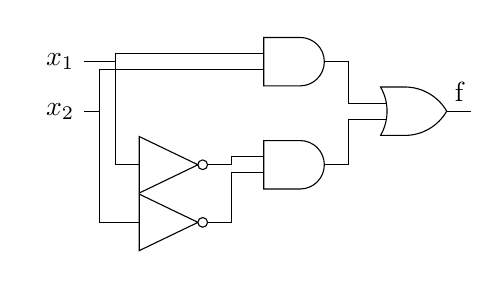
\begin{tikzpicture}[circuit logic US]
    \matrix[column sep=7mm]{
      \node (i1) {$x_1$}; & & \node [and gate] (x1nx2) {}; & \\
      \node (i2) {$x_2$}; &  &  &  \node [or gate] (f) {}; \\
       & \node [not gate] (n1) {}; & \node [and gate] (nx1x2) {};&  \\
      & \node [not gate] (n2) {}; &  & \\
    };
    \draw (i1.east) -- ++(right:4mm) |- (n1.input);
    \draw (i2.east) -- ++(right:2mm) |- (n2.input);

    \draw (i1.east) -- ++(right:4mm) |- (x1nx2.input 1);
    \draw (i2.east) -- ++(right:2mm) |- (x1nx2.input 2);

    \draw (n1.output) -- ++(right:3mm) |- (nx1x2.input 1);
    \draw (n2.output) -- ++(right:3mm) |- (nx1x2.input 2);

    \draw (x1nx2.output) -- ++(right:3mm) |- (f.input 1);
    \draw (nx1x2.output) -- ++(right:3mm) |- (f.input 2);

    \draw (f.output) to [edge label=f] ++(right:3mm);
  \end{tikzpicture}
\end{prob}
\vspace{10em}

\begin{example}
  Convert the following Boolean expression into a network, a truth
  table and a Venn diagram:\\
  \[ f = x_1 \bar{x}_2 + \bar{x}_1 x_2 \]
\end{example}
\vspace{20em}

\begin{prob}
Can two different circuits have the same truth table? Can two different truth tables
have the same circuit? Consider the following two circuits for example \\
\noindent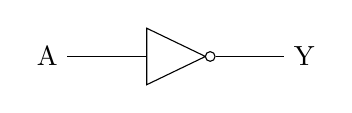
\begin{tikzpicture}[circuit logic US]
  \node (A) {A}; \node [not gate, right=of A] (notA) {}; \node [right=of notA] (Y) {Y};
  \draw (A) -- (notA.input);
  \draw (notA.output) -- (Y);
\end{tikzpicture}\\[1em]

\noindent\begin{tikzpicture}[circuit logic US]
  \node (A) {A}; \node [not gate, right=of A] (notA1) {};
  \draw (A) -- (notA.input);

  \node [not gate, right=of notA1] (notA2) {};
  \draw (notA1.output) -- (notA2.input);

  \node [not gate, right=of notA2] (notA3) {};
  \draw (notA2.output) -- (notA3.input);

  \node [right=of notA3] (Y) {Y};
  \draw (notA3.output) -- (Y);
\end{tikzpicture}

How about Venn digrams?
\end{prob}
\vspace{10em}

\begin{remark}
  Truth tables and Venn diagrams define \emph{what} the combinational circuit should do. Truth tables
  define output for every input.
  Boolean expression and networks define \emph{how} to achieve the desired input
  output relationship.
\end{remark}


\section{Multi-input networks}
\begin{example}
  Convert the following (ANSI) network into a Boolean expression and a truth table.
  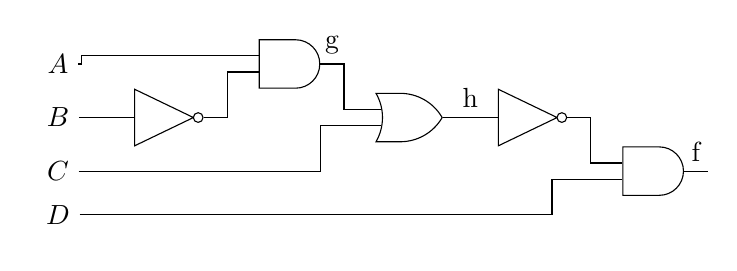
\begin{tikzpicture}[circuit logic US]
    \matrix[column sep=7mm]{
      \node (A) {$A$}; & &  \node [and gate] (andAB) {}; & & & \\
      \node (B) {$B$}; & \node [not gate] (nB) {};  &  & \node [or gate] (orGC) {}; & \node [not gate] (notH) {}; & \\
      \node (C) {$C$}; & & \node (C2) {}; & & & \node [and gate] (andHD) {}; \\
      \node (D) {$D$}; & &  & & \node (D2) {}; &\\
    };
    \draw (A) -- ++(right:3mm) |- (andAB.input 1);
    \draw (B) -- (nB.input);
    \draw (nB.output) -- ++(right:3mm) |- (andAB.input 2);

    \draw (andAB.output) to [edge label=g] ++(right:3mm) |- (orGC.input 1);
    \draw (C) -- (C2.east) -- ++(right:3mm) |- (orGC.input 2);

    \draw (orGC.output)  to [edge label=h] (notH.input);

    \draw (notH.output) -- ++(right:3mm) |- (andHD.input 1);
    \draw (D) -- (D2.east) -- ++(right:3mm) |- (andHD.input 2);
    
    \draw (andHD.output) to [edge label=f] ++(right:3mm);
  \end{tikzpicture}
\end{example}
\vspace{20em}

\begin{prob}
  Convert the following (ANSI) network into a Boolean expression and a truth table.
  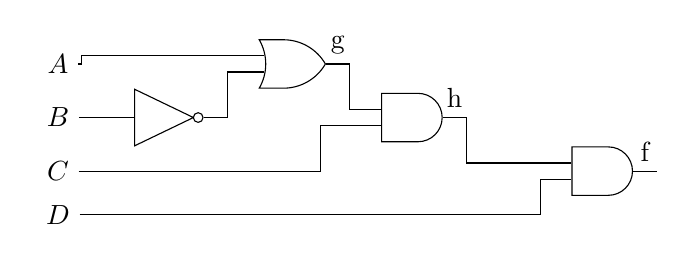
\begin{tikzpicture}[circuit logic US]
    \matrix[column sep=7mm]{
      \node (A) {$A$}; & &  \node [or gate] (andAB) {}; & & & \\
      \node (B) {$B$}; & \node [not gate] (nB) {};  &  & \node [and gate] (orGC) {}; &  & \\
      \node (C) {$C$}; & & \node (C2) {}; & & & \node [and gate] (andHD) {}; \\
      \node (D) {$D$}; & &  & & \node (D2) {}; &\\
    };
    \draw (A) -- ++(right:3mm) |- (andAB.input 1);
    \draw (B) -- (nB.input);
    \draw (nB.output) -- ++(right:3mm) |- (andAB.input 2);

    \draw (andAB.output) to [edge label=g] ++(right:3mm) |- (orGC.input 1);
    \draw (C) -- (C2.east) -- ++(right:3mm) |- (orGC.input 2);

    %\draw (orGC.output)  to [edge label=h] (andHD.input);

    \draw (orGC.output) to [edge label=h] ++(right:3mm) |- (andHD.input 1);
    \draw (D) -- (D2.east) -- ++(right:3mm) |- (andHD.input 2);
    
    \draw (andHD.output) to [edge label=f] ++(right:3mm);
  \end{tikzpicture}
\end{prob}
\vspace{20em}

\section{Minterms and Maxterms}
\subsection{Minterms}
Minterm is a product involving all inputs (or complements) to a function.
Every row of a truth table has a corresponding minterm.
Minterm is true if and only if the corresponding row in the table is active.

Minterms defined as follows for each row of a two input truth table:\\
\begin{tabular}{rrrp{20mm}}
  \toprule
  A & B &  minterm & minterm name\\
  \midrule
  0 & 0 &  $\bar{A} \bar{B}$ & $m_0$ \\
  0 & 1 &  $\bar{A}      B $ & $m_1$ \\
  1 & 0 &  $     A  \bar{B}$ & $m_2$ \\
  1 & 1 &  $     A       B $ & $m_3$ \\
  \bottomrule
\end{tabular}\\[1em]

\noindent Consider a two input circuit whose output $Y$ is given by the truth table:\\
\begin{tabular}{rrrrp{20mm}}
  \toprule
  A & B &  Y & minterm & minterm name\\
  \midrule
  0 & 0 & 0 & $\bar{A} \bar{B}$ & $m_0$ \\
  0 & 1 & 1 & $\bar{A}      B $ & $m_1$ \\
  1 & 0 & 0 & $     A  \bar{B}$ & $m_2$ \\
  1 & 1 & 1 & $     A       B $ & $m_3$ \\
  \bottomrule
\end{tabular}\\[1em]
then $Y = \bar{A}      B  + A B = m_1 + m_3 = \sum (1, 3)$.

\noindent This also gives the \emph{sum of products canonical form}.

\begin{example}
  What is the minterm $m_{13}$ for a 4-input circuit with inputs $x, y, z, w$
  (ordered from MSB to LSB).
\end{example}
\vspace{10em}

%\noindent Find the minterm $m_n$
%\begin{enumerate}
%    \item Convert the minterm number $n$ to a $m$-bit binary number where $m$ is the
%      order of inputs.
%    \item Replace 0 with the corresponding input complement and 1 with the input.
%\end{enumerate}

\begin{prob}
  What is the minterm $m_{23}$ for a 5-input circuit with inputs $a, b, c, d, e$
  (ordered from MSB to LSB).
\end{prob}
\vspace{10em}

\begin{example}
  Convert the following 4-input truth table into sum of minterms and sum of products canonical form.

  \noindent \begin{tabular}{p{20mm}llll|l}
    \toprule
    minterm name & A & B & C & D & f \\
    \midrule
    $m_0$ & 0 & 0 & 0 & 0 & 0 \\ 
    $m_1$ & 0 & 0 & 0 & 1 & 1 \\ 
    $m_2$ & 0 & 0 & 1 & 0 & 0 \\ 
    $m_3$ & 0 & 0 & 1 & 1 & 0 \\ 
    $m_4$ & 0 & 1 & 0 & 0 & 0 \\ 
    $m_5$ & 0 & 1 & 0 & 1 & 1 \\ 
    $m_6$ & 0 & 1 & 1 & 0 & 0 \\ 
    $m_7$ & 0 & 1 & 1 & 1 & 0 \\ 
    $m_8$ & 1 & 0 & 0 & 0 & 0 \\ 
    $m_9$ & 1 & 0 & 0 & 1 & 0 \\ 
    $m_{10}$ & 1 & 0 & 1 & 0 & 0 \\
    $m_{11}$ & 1 & 0 & 1 & 1 & 0 \\
    $m_{12}$ & 1 & 1 & 0 & 0 & 0 \\
    $m_{13}$ & 1 & 1 & 0 & 1 & 1 \\
    $m_{14}$ & 1 & 1 & 1 & 0 & 0 \\
    $m_{15}$ & 1 & 1 & 1 & 1 & 0 \\
    \bottomrule
  \end{tabular}
\end{example}

\begin{prob}
  Convert the following 4-input truth table into sum of minterms and sum of products canonical form.

  \noindent
  \begin{tabular}{p{20mm}llll|l}
    \toprule
    minterm name & A & B & C & D & f \\
    \midrule
    $m_0$ & 0 & 0 & 0 & 0 & 0 \\ 
    $m_1$ & 0 & 0 & 0 & 1 & 0 \\ 
    $m_2$ & 0 & 0 & 1 & 0 & 0 \\ 
    $m_3$ & 0 & 0 & 1 & 1 & 1 \\ 
    $m_4$ & 0 & 1 & 0 & 0 & 0 \\ 
    $m_5$ & 0 & 1 & 0 & 1 & 0 \\ 
    $m_6$ & 0 & 1 & 1 & 0 & 0 \\ 
    $m_7$ & 0 & 1 & 1 & 1 & 1 \\ 
    $m_8$ & 1 & 0 & 0 & 0 & 0 \\ 
    $m_9$ & 1 & 0 & 0 & 1 & 0 \\ 
    $m_{10}$ & 1 & 0 & 1 & 0 & 0 \\
    $m_{11}$ & 1 & 0 & 1 & 1 & 1 \\
    $m_{12}$ & 1 & 1 & 0 & 0 & 0 \\
    $m_{13}$ & 1 & 1 & 0 & 1 & 1 \\
    $m_{14}$ & 1 & 1 & 1 & 0 & 1 \\
    $m_{15}$ & 1 & 1 & 1 & 1 & 0 \\
    \bottomrule
  \end{tabular}
\end{prob}


\subsection{Maxterms}
Maxterm is a sum involving all inputs (or complements) to a function.
Every row of a truth table has a corresponding maxterm.
Minterm is false if and only if the corresponding row in the table is active.

Maxterms are defined as follows for each row of a two input truth table:\\
\begin{tabular}{rrrp{20mm}}
  \toprule
  A & B &  maxterm & maxterm name\\
  \midrule
  0 & 0 &  $A + B$ & $M_0$ \\
  0 & 1 &  $A + \bar{B} $ & $M_1$ \\
  1 & 0 &  $\bar{A} + B$ & $M_2$ \\
  1 & 1 &  $\bar{A} + \bar{B} $ & $M_3$ \\
  \bottomrule
\end{tabular}\\[1em]

\noindent Consider a two input circuit whose output $Y$ is given by the truth table:\\
\begin{tabular}{rrrrp{20mm}}
  \toprule
  A & B &  Y & maxterm & maxterm name\\
  \midrule
  0 & 0 &  0 & $A + B$ & $M_0$ \\
  0 & 1 &  1 & $A + \bar{B} $ & $M_1$ \\
  1 & 0 &  0 & $\bar{A} + B$ & $M_2$ \\
  1 & 1 &  1 & $\bar{A} + \bar{B} $ & $M_3$ \\
  \bottomrule
\end{tabular}\\[1em]
then $Y = (A+B)(\bar{A} + B) = M_0M_2$.

\noindent Writing a functional specification in terms of minterms is also called
product of sums canonical form.

\begin{example}
  Write the maxterm $M_{11}$ for 4-input Boolean function with the ordered inputs $A, B, C, D$.
\end{example}

% \noindent Find the maxterm $M_n$
% \begin{enumerate}
% \item Convert the maxterm number $n$ to a $m$-bit binary number where $m$ is the
%   order of inputs.
% \item Replace 0 with the corresponding input and 1 with the input complement.
% Add + between each input.
% \end{enumerate}

\begin{example}
  Convert the following 4-input truth table into product of maxterms and product of sums canonical form.

  \noindent
  \begin{tabular}{p{20mm}llll|l}
    \toprule
    maxterm name & A & B & C & D & f \\
    \midrule
    $M_0$ & 0 & 0 & 0 & 0 & 0 \\ 
    $M_1$ & 0 & 0 & 0 & 1 & 0 \\ 
    $M_2$ & 0 & 0 & 1 & 0 & 0 \\ 
    $M_3$ & 0 & 0 & 1 & 1 & 1 \\ 
    $M_4$ & 0 & 1 & 0 & 0 & 0 \\ 
    $M_5$ & 0 & 1 & 0 & 1 & 0 \\ 
    $M_6$ & 0 & 1 & 1 & 0 & 0 \\ 
    $M_7$ & 0 & 1 & 1 & 1 & 1 \\ 
    $M_8$ & 1 & 0 & 0 & 0 & 0 \\ 
    $M_9$ & 1 & 0 & 0 & 1 & 0 \\ 
    $M_{10}$ & 1 & 0 & 1 & 0 & 0 \\
    $M_{11}$ & 1 & 0 & 1 & 1 & 1 \\
    $M_{12}$ & 1 & 1 & 0 & 0 & 0 \\
    $M_{13}$ & 1 & 1 & 0 & 1 & 1 \\
    $M_{14}$ & 1 & 1 & 1 & 0 & 1 \\
    $M_{15}$ & 1 & 1 & 1 & 1 & 0 \\
    \bottomrule
  \end{tabular}
\end{example}

\begin{prob}
  Convert the following 4-input truth table into product of maxterms and products of sums canonical form.

  \noindent
  \begin{tabular}{p{20mm}llll|l}
    \toprule
    maxterm name & A & B & C & D & f \\
    \midrule
    $M_0$ & 0 & 0 & 0 & 0 & 0 \\ 
    $M_1$ & 0 & 0 & 0 & 1 & 1 \\ 
    $M_2$ & 0 & 0 & 1 & 0 & 1 \\ 
    $M_3$ & 0 & 0 & 1 & 1 & 1 \\ 
    $M_4$ & 0 & 1 & 0 & 0 & 1 \\ 
    $M_5$ & 0 & 1 & 0 & 1 & 0 \\ 
    $M_6$ & 0 & 1 & 1 & 0 & 1 \\ 
    $M_7$ & 0 & 1 & 1 & 1 & 1 \\ 
    $M_8$ & 1 & 0 & 0 & 0 & 0 \\ 
    $M_9$ & 1 & 0 & 0 & 1 & 1 \\ 
    $M_{10}$ & 1 & 0 & 1 & 0 & 1 \\
    $M_{11}$ & 1 & 0 & 1 & 1 & 1 \\
    $M_{12}$ & 1 & 1 & 0 & 0 & 0 \\
    $M_{13}$ & 1 & 1 & 0 & 1 & 1 \\
    $M_{14}$ & 1 & 1 & 1 & 0 & 1 \\
    $M_{15}$ & 1 & 1 & 1 & 1 & 0 \\
    \bottomrule
  \end{tabular}
\end{prob}

\begin{example}
  Write the 3-input truth table for the function $f = m_2 + m_3 + m_7$.
\end{example}
\vspace{10em}

\begin{prob}
  Write the 3-input truth table for the function $f = M_4M_5M_7$. 
\end{prob}
\vspace{10em}

\begin{prob}
  Write the truth table for the function $f = \bar{A}B\bar{C} + AB\bar{C}$. 
\end{prob}
\vspace{10em}

\section{More Gates and notations summary}
\rotatebox[origin=c]{90}{
\begin{tabular}{lccp{0.2\linewidth}cp{0.2\linewidth}}
  \toprule
  Name & C/Verilog & Boolean expr. & Truth Table & (ANSI) symbol & K-map \\
  \midrule
  NAND Gate &
  \texttt{Q = \~{}(x1 \& x2)} &
  $Q = \overline{x_1 \cdot x_2} = \overline{x_1 x_2}$ &
 \mbox{\begin{tabular}{cc|c}
 \toprule
 $x_1$ & $x_2$ & $\overline{x_1 \cdot x_2}$ \\
 \midrule
 0 & 0 & 1 \\
 0 & 1 & 1 \\
 1 & 0 & 1 \\
 1 & 1 & 0 \\
 \bottomrule
 \end{tabular}} &
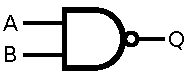
\includegraphics[width=0.2\linewidth]{NAND_ANSI_Labelled.pdf} &
\begin{minipage}[b][][t]{\linewidth}
\begin{Karnaughquatre}
\minterms{0,1,2}
\maxterms{3}
\end{Karnaughquatre}
\end{minipage}
\\
  NOR Gate &
\texttt{Q = \~{}(x1 | x2)} &
$Q = \overline{x_1 + x_2}$ &
\mbox{\begin{tabular}{cc|c}
  \toprule
  $x_1$ & $x_2$ & $\overline{x_1 + x_2}$ \\
  \midrule
  0 & 0 & 1 \\
  0 & 1 & 0 \\
  1 & 0 & 0 \\
  1 & 1 & 0 \\
  \bottomrule
\end{tabular}} &
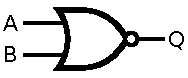
\includegraphics[width=0.2\linewidth]{NOR_ANSI_Labelled.pdf} & 
                                                               \begin{minipage}[b][][t]{\linewidth}
\begin{Karnaughquatre}
\minterms{3}
\maxterms{0,1,2}
\end{Karnaughquatre}
\end{minipage}
\\
XOR Gate &
\texttt{Q = x1 \^{} x2}
&
$ Q = x_1 \oplus x_2$
&
\mbox{\begin{tabular}{cc|c}
\toprule
$x_1$ & $x_2$ & $x_1 \oplus x_2$ \\
\midrule
0 & 0 & 0 \\
0 & 1 & 1 \\
1 & 0 & 1 \\
1 & 1 & 0 \\
\bottomrule
        \end{tabular}}
&
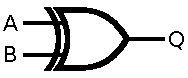
\includegraphics[width=0.2\linewidth]{XOR_ANSI_Labelled.pdf} &
\begin{minipage}[b][][t]{\linewidth}
\begin{Karnaughquatre}
\minterms{1,2}
\maxterms{0,3}
\end{Karnaughquatre}
\end{minipage}
\\
XNOR Gate &
\texttt{Q = \~{}(x1 \^{} x2)}
&
$ Q = \overline{x_1 \oplus x_2}$
&
\mbox{\begin{tabular}{cc|c}
        \toprule
        $x_1$ & $x_2$ & $\overline{x_1 \oplus x_2}$ \\
        \midrule
        0 & 0 & 1 \\
        0 & 1 & 0 \\
        1 & 0 & 0 \\
        1 & 1 & 1 \\
        \bottomrule
      \end{tabular}}
    &
    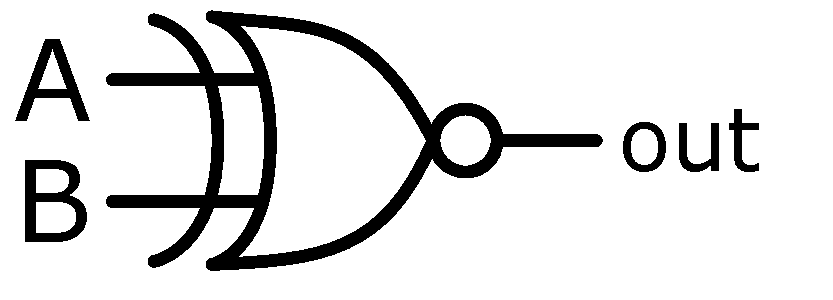
\includegraphics[width=0.2\linewidth]{XNOR_ANSI_Labelled.pdf} &
    \begin{minipage}[b][][t]{\linewidth}
      \begin{Karnaughquatre}
        \minterms{0,3}
        \maxterms{1,2}
      \end{Karnaughquatre}
    \end{minipage}
  \end{tabular}
}
\newpage

\section{Boolean Algebra}

\subsection{Axioms of Boolean algebra}

\begin{enumerate}
\item 
  $ 0 \cdot 0 = 0 $
\item 
    $ 1 + 1 = 1 $
\item
    $ 1 \cdot 1 = 1 $
\item
    $ 0 + 0 = 0 $
\item
    $ 0 \cdot 1 = 1 \cdot 0 = 0 $
\item
      $ \bar{0} = 1 $
\item
        $ \bar{1} = 0 $
\item
      $ x = 0 \text{ if } x \ne 1$ 
    \item
      $ x = 1 \text{ if } x \ne 0$ 
\end{enumerate}

\subsection{Single variable theorems}

\begin{enumerate}
\item $ x \cdot 0 = 0 $
  \vspace{5em}
\item $ x + 1 = 1 $
  \vspace{5em}
\item $ x \cdot 1 = x $
  \vspace{5em}
\item $ x + 0 = x $
  \vspace{5em}
\item $ x \cdot x = x $
  \vspace{5em}
\item $ x + x = x $
  \vspace{5em}
\item $ x \cdot \bar{x} = 0 $
  \vspace{5em}
\item $ x + \bar{x} = 1 $
  \vspace{5em}
\item $\bar{\bar{x}} = x $
  \vspace{5em}
\end{enumerate}

\begin{remark}[Duality]
  Swap $+$ with $\cdot$ and 0 with 1 to get another theorem
\end{remark}

\subsection{Two and three variable properties}

\begin{enumerate}
\item Commutative: $x\cdot y = y \cdot x$ , $x + y = y + x$
  \vspace{10em}
\item Associative: $x\cdot(y\cdot z) = (x \cdot y) \cdot z$, $x+(y+ z) = (x + y) + z$
  \vspace{10em}
\item Distributive: $x\cdot(y + z) = x \cdot y + x \cdot z$, $x + y \cdot z = (x + y) \cdot (y + z)$
  \vspace{10em}
\item Absorption: $x + x\cdot y = x$, $x \cdot (x+y) = x$
  \vspace{10em}
\item Combining: $x \cdot y + x \cdot \bar{y}$, $(x+y) \cdot (x + \bar{y}) = x$
  \vspace{10em}
\item DeMorgan's theorem: $\overline{x \cdot y} = \bar{x} + \bar{y}$,
  $\overline{x + y} = \bar{x} \cdot \bar{y}$.
  \vspace{10em}
\item Concensus:
  \begin{enumerate}
  \item $x + \bar{x}\cdot y = x + y$
    \vspace{10em}
  \item $x \cdot (\bar{x} + y) = x \cdot y$
    \vspace{10em}
  \item $x \cdot y + y\cdot z + \bar{x} \cdot z = x\cdot y + \bar{x} \cdot z$
    \vspace{10em}
  \item $(x + y) \cdot (y+ z) \cdot (\bar{x} + z) = (x+ y) \cdot (\bar{x} + z)$
    \vspace{10em}
  \end{enumerate}
\end{enumerate}

\begin{example}[Multiplexer]
  Multiplexer is a circuit used to select one of the input lines $x_1$ and $x_2$
  based only select input $s$. When $s=0$, $x_1$ is selected, $x_2$ is selected otherwise.
  Find a boolean expression and a circuit for multiplexer\\
  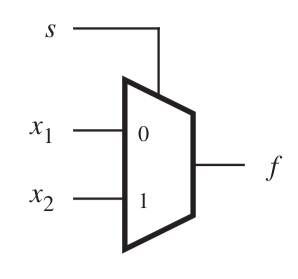
\includegraphics[width=0.2\linewidth]{multiplexer-symbol.png}
  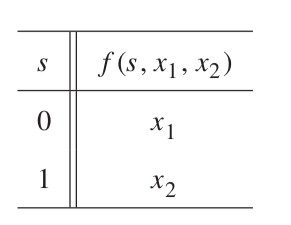
\includegraphics[width=0.2\linewidth]{multiplexer-spec.png}
\end{example}
\vspace{10em}

\begin{example}
  Simplify $f = \bA\bB\bC + A \bB\bC + A\bB\bC $ using boolean algebra.
\end{example}
\vspace{10em}

\begin{example}
  Simplify $f = \bA\bA\bC + \bA\bB C $ using K-maps.
\end{example}
\vspace{10em}


%\bibliography{main}
%\bibliographystyle{plain}
\end{document}
